\section{Balance of Nature} \index{Nature, balance of}

\begin{multicols}{2}


%==================================================================================================%

\section*{The Natural Environment}


\subsection{Camouflage and Protection} \index{Camouflage} % VSO 57

\begin{center}
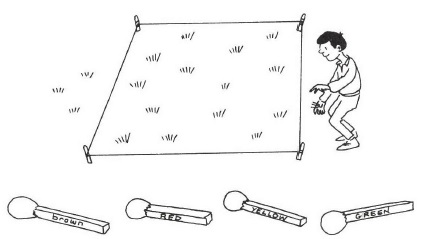
\includegraphics[width=0.45\textwidth]{./img/vso/camouflage-protection.jpg}
\end{center}

\begin{description*}
%\item[Subtopic:]{}
\item[Materials:]{Long piece of string, 4 pegs, matches, marker pens}
%\item[Setup:]{}
\item[Procedure:]{Mark out an area of grass with
the string and pegs. Colour the
matchsticks with markers. Make some the same
colour as the grass and others
very bright. Drop the
matches over the area of grass.
}
%\item[Hazards:]{}
%\item[Questions:]{Which matches are easiest to
%find?}
\item[Observations:]{The green matches blend into their surroundings and hence are safer from predators.}
%\item[Theory:]{}
%\item[Applications:]{Discuss with students why
%camouflage would be an
%advantage to a small maggot and
%why it would help a predator too.}
\item[Notes:]{Alternatively, cut moth shapes from newspaper
and white paper and place both types on either kind of paper. Which are easier to see?}
\end{description*}

\subsection{Reactions to Light} % VSO 57

\begin{center}
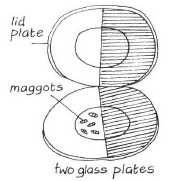
\includegraphics[width=0.35\textwidth]{./img/vso/reactions-light.jpg}
\end{center}

\begin{description*}
%\item[Subtopic:]{}
\item[Materials:]{2 plates, maggots}
%\item[Setup:]{}
\item[Procedure:]{Paint or cover one half of each of
the plates. Put the plates together
so that half is dark and half in
bright light. Put 10 maggots into
the centre of the bottom plate
and put the `lid' back. Count how
many maggots are in each side
every 10 minutes.}
%\item[Hazards:]{}
%\item[Questions:]{}
\item[Observations:]{The maggots prefer the light.}
%\item[Theory:]{}
%\item[Applications:]{}
%\item[Notes:]{}
\end{description*}

\columnbreak

\subsection{Reactions to Humidity} \index{Humidity}

\begin{center}
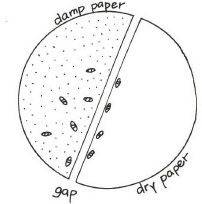
\includegraphics[width=0.25\textwidth]{./img/vso/reactions-humidity.jpg}
\end{center}

\begin{description*}
%\item[Subtopic:]{}
\item[Materials:]{Plate, toilet paper, cloth}
%\item[Setup:]{}
\item[Procedure:]{Put dry toilet paper on one side of
a plate and damp paper on the
other. Put a plate on top and
cover it with a cloth so it is dark
underneath. Count how many
maggots are on each side every
10 minutes.}
%\item[Hazards:]{}
%\item[Questions:]{}
\item[Observations:]{The maggots prefer a humid environment.}
%\item[Theory:]{}
\item[Applications:]{Investigate several conditions at
once. For example, put damp
filter paper on one half of the 2
plates. Is the result the same if
both plates are in sunlight? Which
is more important, dampness or
darkness?}
%\item[Notes:]{}
\end{description*}

%\subsection{Disappearing Moths} % VSO 57
%
%%\begin{center}
%%\includegraphics[width=0.4\textwidth]{./img/.png}
%%\end{center}
%
%\begin{description*}
%%\item[Subtopic:]{}
%\item[Materials:]{Newspaper, white paper}
%%\item[Setup:]{}
%\item[Procedure:]{Cut moth shapes from newspaper
%and white paper. Place both types
%of moth onto newspaper, and
%then onto white paper. Note
%which moths are easier to see.}
%%\item[Hazards:]{}
%%\item[Questions:]{}
%%\item[Observations:]{}
%%\item[Theory:]{}
%%\item[Applications:]{}
%%\item[Notes:]{}
%\end{description*}

\subsection{Aquarium} \index{Aquarium} % Shika 227 

\begin{center}
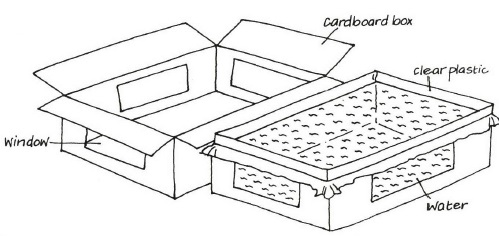
\includegraphics[width=0.49\textwidth]{./img/vso/aquarium.jpg}
\end{center}

\begin{description*}
%\item[Subtopic:]{}
\item[Materials:]{Cardboard box, clear plastic, tape, scissors, water}
%\item[Setup:]{}
\item[Procedure:]{Cut viewing windows in the sides of a box. Line the box with a large sheet of clear plastic and fill it with water. Attach the plastic firmly around the edges (e.g. with tape).}
%\item[Hazards:]{}
%\item[Questions:]{}
%\item[Observations:]{}
\item[Theory:]{Unlike the terrarium, the aquarium is not sustainable because aquatic organisms often require more oxygen dissolved  in the water than the container can hold. Adding aquatic plants increases the amount of oxygen in the aquarium.}
%\item[Applications:]{}
%\item[Notes:]{}
\end{description*}

\columnbreak

%\subsection{Ant Farm} % Shika 227 PIC!!!
%
%%\begin{center}
%%\includegraphics[width=0.4\textwidth]{./img/.png}
%%\end{center}
%
%\begin{description*}
%%\item[Subtopic:]{}
%\item[Materials:]{}
%\item[Setup:]{}
%\item[Procedure:]{Place a }
%\item[Hazards:]{}
%\item[Questions:]{}
%\item[Observations:]{}
%\item[Theory:]{}
%\item[Applications:]{}
%\item[Notes:]{}
%\end{description*}

\subsection{Terrarium} \index{Terrarium} % Shika 227 VSO 123 pic

\begin{center}
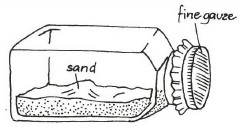
\includegraphics[width=0.4\textwidth]{./img/vso/terrarium.jpg}
\end{center}

\begin{description*}
%\item[Subtopic:]{}
\item[Materials:]{Square plastic bottle, sand, soil, rocks, plants, insects, fine gauze}
%\item[Setup:]{}
\item[Procedure:]{Cut a square plastic bottle in half lengthwise. Fill one side with soil, rocks, sticks, moss, insects, etc. and cover and tape with the top half. Poke a few holes for air to enter. Periodically add water by removing and replacing the top lid.}
%\item[Hazards:]{}
%\item[Questions:]{}
%\item[Observations:]{}
%\item[Theory:]{}
%\item[Applications:]{}
%\item[Notes:]{}
\end{description*}

%==================================================================================================%

\section*{Interaction of Living and \hfill \\ Non-Living Things} \index{Living things! interaction of}


\subsection{Carbon Cycle Cards} \index{Carbon cycle} \index{Storage} % VSO 56

\begin{center}
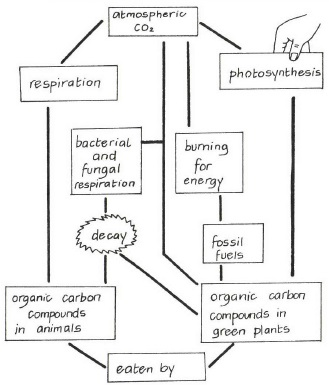
\includegraphics[width=0.45\textwidth]{./img/vso/carbon-cycle.jpg}
\end{center}

\begin{description*}
%\item[Subtopic:]{}
\item[Materials:]{Cards, paper strips, string}
%\item[Setup:]{}
\item[Procedure:]{Cut out cards showing stages of
the carbon cycle. Link them
together with the paper strips or string to
make a balanced carbon cycle.
Discuss with students the
consequences of increasing one
stage, e.g. burning extra fossil
fuels.}
%\item[Hazards:]{}
%\item[Questions:]{}
%\item[Observations:]{}
%\item[Theory:]{}
%\item[Applications:]{}
\item[Notes:]{Cards can be made for other cycles as well (e.g. water cycle, nitrogen cycle).}
\end{description*}

\columnbreak

\subsection{Water Cycle} \index{Water! cycle} \index{Storage}

\begin{center}
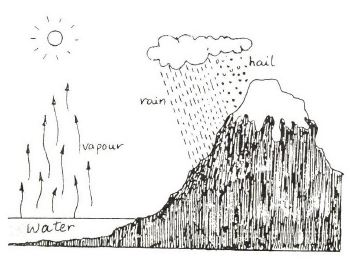
\includegraphics[width=0.49\textwidth]{./img/source/water-cycle.jpg}
\end{center}

\begin{description*}
%\item[Subtopic:]{}
\item[Materials:]{Cards, paper strips, string}
%\item[Setup:]{}
\item[Procedure:]{Prepare activity cards as with the carbon cycle.}
%\item[Hazards:]{}
%\item[Questions:]{}
%\item[Observations:]{}
%\item[Theory:]{}
%\item[Applications:]{}
%\item[Notes:]{}
\end{description*}

\subsection{Nitrogen Cycle} \index{Nitrogen! cycle} \index{Storage}

\begin{center}
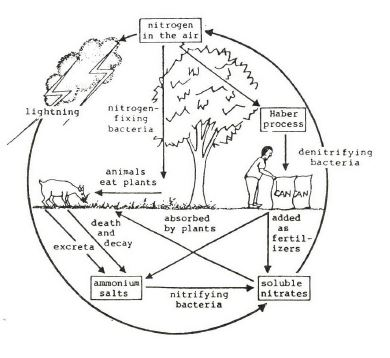
\includegraphics[width=0.49\textwidth]{./img/source/nitrogen-cycle.jpg}
\end{center}

\begin{description*}
%\item[Subtopic:]{}
\item[Materials:]{Cards/manila, flip chart}
%\item[Setup:]{}
\item[Procedure:]{Prepare a wall chart of the natural nitrogen
circulation or make cards of the various steps for students to place. }
%\item[Hazards:]{}
%\item[Questions:]{}
%\item[Observations:]{}
\item[Theory:]{When proteins are broken down in
the body, combined nitrogen containing
compounds leave the body with the urine. These
compounds are broken down further by bacteria
to ammonia (NH$_4$) which makes
public places of urination smell very badly.
Dead plant and animal tissues are similarly
broken down. The ammonia formed is washed
into the soil, where it is acted upon by different
types of bacteria, eventually converting it into
nitrates and ammonium salts which are needed
by plants to produce proteins. Hence they are
important fertilizers.}
%\item[Applications:]{}
%\item[Notes:]{}
\end{description*}

\columnbreak

%==================================================================================================%

\section*{Food Chains and Food Webs} \index{Food chains} \index{Food webs}


\subsection{Food Chain Links} % VSO 56

\begin{center}
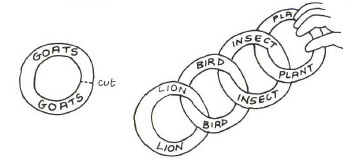
\includegraphics[width=0.45\textwidth]{./img/vso/food-chain-links.jpg}
\end{center}

\begin{description*}
%\item[Subtopic:]{}
\item[Materials:]{Cardboard, scissors}
%\item[Setup:]{}
\item[Procedure:]{Cut links of the food chain from
stiff cardboard. Label each link
with one part of the food chain.
Put the links together to make a
chain. Make both simple and more complicated chains.}
%\item[Hazards:]{}
\item[Questions:]{What happens if one link in the middle is removed?}
\item[Observations:]{If a middle link is removed, many other links are impacted.}
\item[Theory:]{Removing a single species can have a dramatic impact on the entire ecosystem.}
%\item[Applications:]{}
%\item[Notes:]{}
\end{description*}

\subsection{Food Webs} % VSO 56

\begin{center}
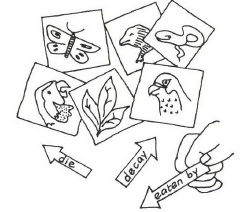
\includegraphics[width=0.4\textwidth]{./img/vso/food-webs.jpg}
\end{center}

\begin{description*}
%\item[Subtopic:]{}
\item[Materials:]{Card, pictures of animals and plants (optional)}
%\item[Setup:]{}
\item[Procedure:]{Either draw pictures of animals
and plants on cards or stick on
pictures cut out from magazines
etc. Make arrows and write on
them the links shown. Arrange
the cards and arrows to make a
food web.}
%\item[Hazards:]{}
%\item[Questions:]{}
%\item[Observations:]{}
%\item[Theory:]{}
%\item[Applications:]{}
%\item[Notes:]{}
\end{description*}

\columnbreak

\subsection{Food Web Connections} % Shika 225

%\begin{center}
%\includegraphics[width=0.4\textwidth]{./img/.png}
%\end{center}

\begin{description*}
%\item[Subtopic:]{}
\item[Materials:]{Long rope/string, students}
%\item[Setup:]{}
\item[Procedure:]{Organize students into a circle. Holding the rope tightly, throw the rope to another student. They pull it tight and throw to another (throws do not need to be adjacent). Once the chain is complete, have one student let go of the rope.}
%\item[Hazards:]{}
%\item[Questions:]{}
%\item[Observations:]{}
\item[Theory:]{The food web represents the different interconnected species in an ecosystem - each student is a member of the food chain. If one species becomes extinct (i.e. one student drops the rope), then it impacts the entire food chain. Other species lose connections (i.e. food) and are in threat of extinction themselves.}
%\item[Applications:]{}
\item[Notes:]{Alternatively, select students to sit down, meaning they have gone extinct as a species. This makes it more difficult for the others to remain standing, i.e. adds strain on their existence.}
\end{description*}

%==================================================================================================%


\end{multicols}

\pagebreak